%!TEX root = ../rapport.tex

\chapter{Spécifications}

Lorsque la STB est enclenchée, celle-ci doit être capable de se connecter à notre serveur.
\section{Globale}
\begin{figure}[H]
    \begin{center}
        \centering 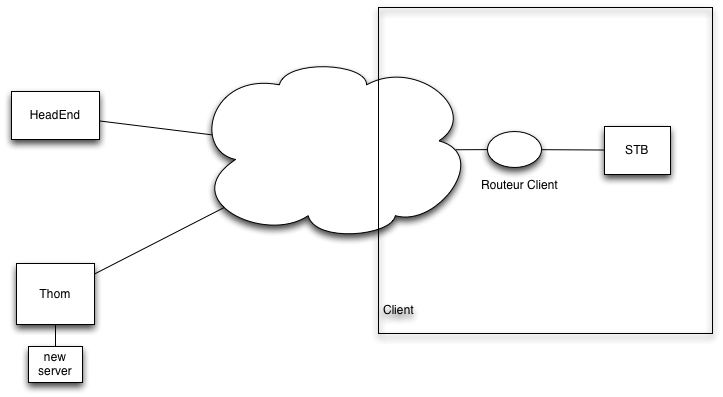
\includegraphics[width=0.7\linewidth]{CDC/schema_comm.png}
        \caption{Schéma}
    \end{center}
\end{figure}

Head End: C'est ici que les chaînes de TV sont reçues, encodées, encryptées et envoyées.

Thom: service de supervision.

Serveur: C'est ici que l'implémentation côté serveur sera déployée.

Nuage: Internet

Partie cliente: Routeur du client, connexion avec la STB qui contient le code android permettant la communication.


\begin{figure}[H]
    \begin{center}
        \centering 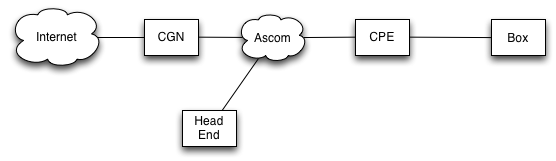
\includegraphics[width=0.7\linewidth]{CDC/schema_comm_client.png}
        \caption{Schéma}
    \end{center}
\end{figure}


CGN: Carrier Grade NAT, utilisé par le FAI afin d'utiliser du NAT, soit transformer un ensemble d'adresse privée en une seule adresse publique, différenciée par le port TCP.

CPE: Customer Promises Equipment, équipement côté client. Il s'agit ici du routeur du client.

\section{Set-Top Box}

La STB utilisée par WinGo est une box tournant sous Android. Il s'agit d'une surcouche graphique se superposant à l'image de la TV, donnant des informations supplémentaires comme la durée restante du programme en cours, le programme par chaînes etc. Il n'est pour le moment pas sûr que la box soit modifiable comme on le souhaite. C'est pourquo



% section structure_du_document (end)